\documentclass[../report.tex]{subfiles}

\begin{document}
\graphicspath{{img/}{../img/}}


\section{Gantt planl�gning}
Gantt er en udbyggelse af den klassiske tidsplan. Den er lavet for at give et bedre overblik over de forskellige planlagte opgaver i forhold til hinanden. Hvor en klassisk tidsplan i form af en tabel er fokuseret p� tidsperioderne, er et Gantt diagram fokuseret p� arbejdsopgaverne.\\

P� side \pageref{fig:Gantt} ses Gantt diagrammet for target projektet. Diagrammet er meget skrabet. Det er pga. den valgte procesmodel, Scrum, hvori aktiviteter opdeles og estimeres l�bende. Gantt diagrammet er alts� lavet p� baggrund af en delvis breakdown(se \ref{sec:Activity Breakdown}) af aktiviteter, og et estimat ikke p� arbejdstimer men et bud p� hvor stor en del af projektet en del-aktivitet kan tage. \\

Havde target projektet brugt en vandsfalds process(se \ref{sec:Waterfall}) kunne man have valgt at lave et fuldt produkt og aktivitets breakdown for s� at estimere det hele og lave Gantt diagrammet.
\\ \\


\begin{figure}[H]
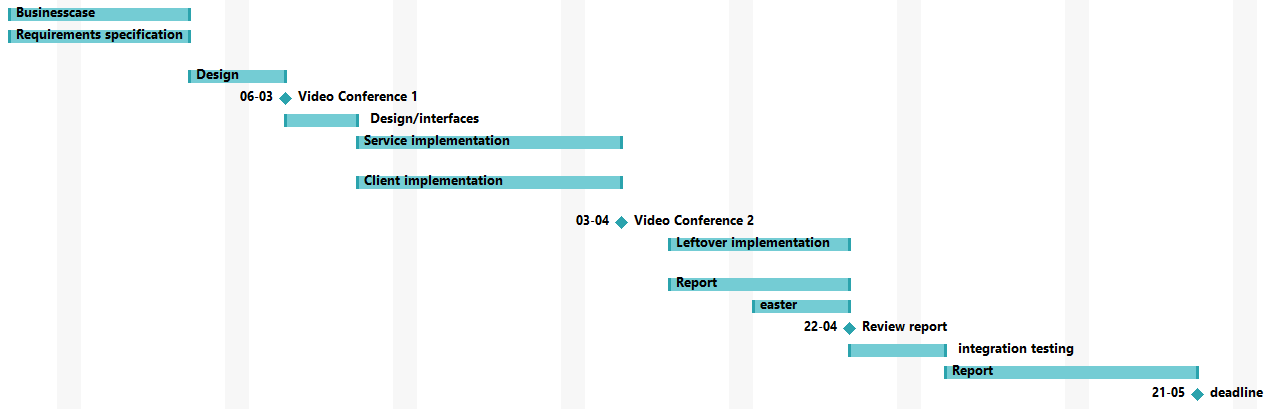
\includegraphics[scale=0.45]{TargetProjectGantt.png}
\label{fig:Gantt}
\end{figure}

Gantt diagrammet vinder stort inden for overblik mod den klassiske tidsplan, men i n�ste kapitel kigges der p� et andet alternativ til aktivitetsplanl�gning.








\end{document}